
\ChapterStar{Introduction}
\begin{refsection}

\addstarredpart{Introduction}
\markboth{Introduction}{INTRODUCTION}
\section*{}
Comprendre la nature et les mécanismes du transport des particules dans un
plasma en présence d'un champ magnétique est une étape essentielle au
développement et à l'optimisation de nombreuses applications.
Parmis les plus ambitieuses, la fusion thermonucléaire contrôlée, qui
consiste à reproduire sur Terre des réactions de fusion\footnote{La réaction de
fusion entre deux atomes d'hydrogène, qui fait naturellement briller les
étoiles, est à ce jour la source d'énergie la plus prometteuse pour soutenir le besoin croissant en énergie de notre civilisation,
économiquement pérenne, techniquement faisable et écologiquement durable.},
repose sur un dispositif de confinement magnétique en forme d'anneau appelé « tokamak ».
La matière, chauffée à des températures supérieures à 150 millions de degrés
Celsius, y est totalement ionisée et doit être confinée par un puissant champ magnétique afin
de rester dans cet état. La réussite de ce projet (d'initiative
internationnale depuis le lancement du programme ITER) dépend alors
fondamentalement de la maîtrise du transport de l'énergie et de la matière au
sein de ce champ magnétique.

Cette problématique, cruciale pour la recherche sur la fusion, est tout aussi
importante dans le développement de sources plasmas froids (avec un plasma
partiellement ionisé dont la température des ions, proche de celle du gaz,
est bien inférieure à la température des électrons : $T_e\neq T_i\sim
T_n$) qui opèrent à basse pression, et dans lesquelles l'application d'un champ
magnétique amène à des améliorations critiques pour les performances de la
décharges. Ce type de source est communément utilisé dans de
nombreux domaines, tels que le traitement et la gravure de
surface~\parencite{Lieberman}, la propulsion spatiale~\parencite{Zhurin}, ou
encore l'injection de neutres pour la fusion~\parencite{SimoninHDR}. Le champ
magnétique permet alors de limiter la pertes des particules sur les parois (miroirs magnétiques,
magnétrons), de laisser pénétrer dans le plasma une tension appliquée
(propulseurs à effet Hall, extraction des ions négatifs), et/ou d'obtenir un
certain type de chauffage par le couplage d'énergie entre des ondes
électromagnétiques et les électrons (décharges hélicons, sources à résonnance
électron-cyclotron (ECR)). Ces sources ont typiquement pour paramètres : une
densité plasma $n_e\sim\,$10$^{16}$ - 10$^{18}\,$m$^{-3}$, une densité de gaz
$n_g\sim\,$10$^{19}\,$m$^{-3}$, une température électronique $T_e\sim\,$1-20~eV,
une intensité de champ magnétique pouvant varier de quelques Gauss à 0.1~Tesla,
et sont donc radicalement différents de ceux des plasmas chaud de fusion.

Le développement et l'optimisation de ces sources se basent généralement sur la
combinaison de recherches expérimentales et d'études théoriques, elles-même
fortement secondées par l'introduction d'un nouveau type d'empirisme : la
simulation numérique.
La construction de codes de calculs, traduisant divers niveaux d'abstraction de
modèles physiques, mathématiques et numériques, et donnant accès à une
certaine réalité virtuelle à questionner, peut nous aider à
comprendre et à interpréter les phénomènes et les processus qui apparaissent dans ces
plasmas. Cependant, dans le domaine des plasmas froids, la compréhension de
l'effet du champ magnétique est loin d'être complète, et les méthodes
habituelles de modélisation, basées sur des hypothèses d'ordering parfois
injustifiées, atteignent leur limites dans le cas des sources basse-pression. 

Ce
problème est devenu particulièrement urgent dans les récents efforts entrepris pour modéliser
la source d'ions négatifs du système d'injection de neutres d'ITER, dans
laquelle le champ magnétique, initialement mis en place pour abaisser la
température électronique et faciliter l'extraction des ions négatifs, entraîne
l'apparition d'un comportement complexe encore mal compris.

\begin{center}
\rule{0.6\textwidth}{1pt}
\end{center}

Le futur réacteur expérimental de fusion ITER se servira de deux injecteurs de
neutres pour chauffer le plasma, générer du courant et alimenter le réacteur en
combustible. Dans le cahier des charges d'ITER, ces injecteurs
sont censés déposer 17~MW de puissance chacun, en accélérant un
faiseau de 40~A d'ions D$^-$ à 1~MeV d'énergie puis en le neutralisant afin de
l'injecter directement dans le plasma de c\oe ur. 
Pour atteindre ces objectifs,
la source d'ions négatifs en amont de l'injecteur doit fournir
une densité de courant de l'ordre de 250~A/m$^2$, uniformément répartie sur une
large surface ($\sim\,$1.6~m x 0.8~m) tout en opérant à
basse-pression (<~0.3~Pa)~\parencite{SimoninHDR}. 

Le concept de source d'ions négatifs retenu pour le projet ITER est
actuellement développé à l'IPP de Garching~\parencite{Hemsworth}. Il s'agit
d'une source à couplage inducif (ICP) dans laquelle la création du plasma et la
production d'ions négatifs prennent place dans deux régions séparées de la
source (schématiquement représentée sur la
figure~\ref{IPPIonSource}). Le plasma est créé par un chauffage radio-fréquence
(RF) de 100 kW à 1MHz dans des "drivers", puis diffuse à travers une chambre
d'expansion rectangulaire. La production d'ions négatifs a lieu quant à elle de
l'autre côté de la source, au niveau des grilles d'extraction, par des
réactions de surface sur les parois vaporisée au césium.
Cette région est séparée de la zone de création du plasma par un filtre magnétique dont le rôle
principal est de réduire la température électronique à proximité de la grille
d'extraction, ce qui est nécéssaire pour obtenir une production suffisante
d'ions négatifs et limiter leur taux de destruction par collision avec les
électrons. 
Depuis quelques années, le développement de la source fait cependant face à un
problème majeur vis-à-vis de la non-uniformité du courant extrait, bien plus
important dans la partie haute de la source que dans sa partie basse. 

\begin{figure}[!hbtp]
\subfigure[]{\label{IPPIonSource}
 \begin{minipage}[c][1\width]{0.5\textwidth} 
 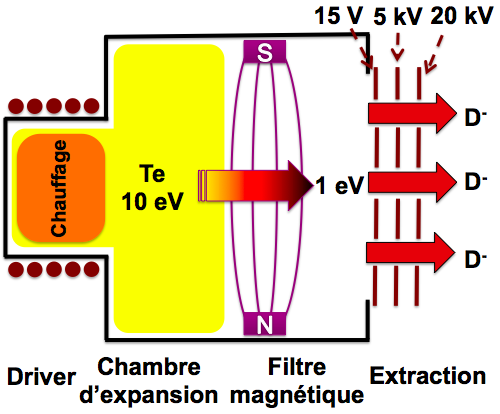
\includegraphics[width=0.8\textwidth]{figures/sourceIPP.png}
 \end{minipage}} 
\subfigure[]{
 \begin{minipage}[c][1\width]{ 0.5\textwidth} 
 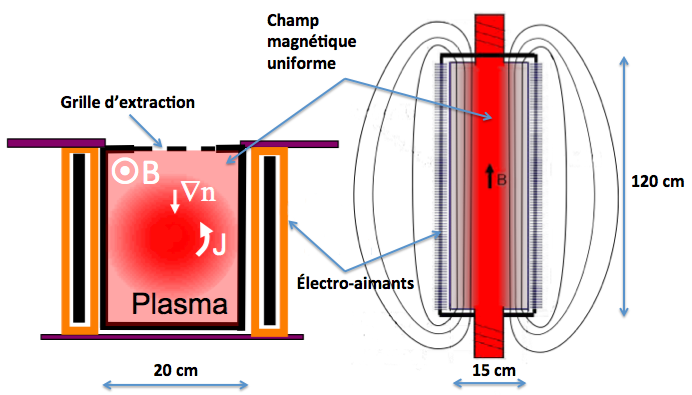
\includegraphics[width=0.8\textwidth]{figures/sourceSimonin1.png}\label{SimoninIonSource}
 \end{minipage}} 
 \caption{Schémas des deux concepts de source d'ions négatifs :
    \subref{IPPIonSource}~ Prototype d'un "driver" de la source IPP de Garching
    ; \subref{SimoninIonSource}~ Source CYBELE en géométrie colonne en
    développement au CEA. } 
 \end{figure}

Pour
comprendre l'origine de ce phénomène et corriger l'inhomogénéité du plasma, de
serieux efforts ont été entrepris, aussi bien au niveau de la modélisation que
de l'expérimentation. Hélas, la physique qui résulte de la combinaison entre le
plasma du driver, de la zone d'extraction et de la zone de filtre est très
complexe, et entraîne l'apparition de forts gradients de densité, de température
et de potentiel eux mêmes responsables 


 Afin d'obtenir une bonne
compréhension de la physique Le groupe GREPHE du LAPLACE a été choisi pour développer un modèle numérique autoconsistant de cette source en 2006

colonnes
\parencite{RosenbluthSimon}
\parencite{Sakawa} (Modified Simon Hoh Instability)$E_r\cdot\nabla n > 0$
\parencite{Hoh} Instability Penning discharge
\parencite{Fruchtman} stationnaire
\parencite{Sternberg} plasma infini dans z, symetrie axiale \ldots 

\parencite{Rosenbluth}\parencite{Chandrasekhar}
\begin{center}
\rule{0.6\textwidth}{1pt}
\end{center}

Le comportement d'un plasma en présence d'un champ magnétique a été
longuement étudié et se trouve maintenant décrit dans de nombreux ouvrages sur
la physique des plasmas.
Les premières expérimentations dans les années 1950-1960 sur le confinement
magnétique du plasma démontrèrent l'existence d'un regime de transport classique
de type diffusif suivant une loi d'échelle en 1/B$^2$, puis, à plus haut champ
magnétique, l'apparition d'un régime de transport anormal variant plutôt en
1/B~\parencite{Bohm,Simon55,Yoshikawa,Janes,Rozhansky}. Les travaux plus
récents sur ce sujet montrent une nette distinction de
comportement entre les plasmas chauds de fusion et les plasmas froids, comme
discuté maintenant.

Pour les plasmas chauds, la littérature est actuellement en grande partie dédiée
à l'étude du transport turbulent et d'une grande variété d'instabilités qui
se développent et dégradent le confinement magnétique. De nombreuses
publications donnent des preuves expérimentales et une caractérisation de ces
phénomènes. Les théories et modèles correspondants sont typiquement basés sur
les approximations suivantes :

\begin{itemize}
  \item L'ionisation (quasiment) totale du plasma
  \item Une agitation thermique importante des les particules
  \item La forte magnétisation des électrons et des ions par un champ de
  plusieurs Teslas confinant le plasma dans un volume fini
  \item L'interaction de type Spitzer (collisions coulombiennes) entre les
  particules
\end{itemize}

Dans les méthodes standards de modélisation, on retrouve les théories fluides de
la Magnéto-hydrodynamique
 (MHD) introduite
par Alfvén~\parencite{Alfven} et des vitesses de dérive~\parencite{SarazinPhD}
ou encore celle du centre-guide pour les modèles
particulaires~\parencite{Taylor,Lee,Garbet10}.
La MHD, généralisation de la mécanique des fluides, assimile le plasma à un fluide unique dans lequel
l'inertie est essentiellement due aux ions et la mobilité reliée aux
électrons~\parencite{Rax}. Du point de vue particulaire, la
théorie du centre-guide décompose le mouvement des particules en un mouvement
circulaire rapide superposé au déplacement d'un centre-guide parallèlement et
perpendiculairement au champ magnétique. L'approche fluide des vitesses de
dérive est quant à elle préférée à partir du moment où les vitesses des deux fluides
ioniques et électroniques diffèrent de trop et qu'il devient plus logique de les
suivre séparément : c'est l'approche que nous étudions dans cette thèse pour
décrire les plasmas de bord des tokamaks.

Dans le domaine des plasmas froids, une autre méthodologie s'est développée du
fait des conditions de plasmas et des intérêts de recherche
différents. En effet, les sources plasmas magnétisées qui nous intéressent
se distinguent des plasmas de fusion sous plusieurs aspects :

\begin{itemize}
  \item Du fait de la faible intensité du champ magnétique (de l'ordre de
  0.01~T), seuls les électrons sont magnétisés, le rayon le Larmor ionique dépassant souvent la
  taille caractéristique du système
  \item La matière n'est que partiellement ionisée, l'interaction avec
  le gaz neutre influençant de façon prédominante le transport dans le plasma.
  \item Le plasma n'est pas confiné sur des lignes de champ fermée et
  l'interaction avec les parois est omniprésente, celles-ci agissant comme de
  parfaits puits de particules et d'énergie pour le plasma ;
  le temp de résidence d'une particule dans le système se voit
  ainsi considérablement diminué et les distributions en vitesses des
  espèces peuvent s'écarter de façon notable de distributions maxwelliennes.
\end{itemize}

Le transport dans ces sources se décrit habituellement par des modèles fluides
de type Dérive-Diffusion~\parencite{Porteous,Lieberman,Rozhansky} quand les
plasmas sont suffisamment collisionnels. Des modèles
cinétiques Particles-In-Cell (PIC) avec des opérateurs collisionnels
Monte-Carlo~\parencite{PIC3D,Adam} ou hybrides
fluide-cinétique~\parencite{BoeufGarrigues} peuvent aussi être utilisés quand
une connaissance détaillée de la fonction de distribution devient nécessaire
(interactions ondes-particules, population à plusieurs niveaux d'énergie), mais
ils requièrent des ressources et des temps de calculs bien plus conséquents que
leurs homologues fluides, ce qui les rend bien moins adaptés aux études
paramétriques. De plus, la plupart de ces travaux de modélisation se focalisent
sur la performance et la caractérisation des décharges pour des applications
spécifiques (\parencite{Lieberman} et reférences inclues) et, excepté quelques
récentes études analytiques de colonnes de plasma idéales
(stationnaires~\parencite{Sternberg}, infinie suivant la direction axiale et de
symétrie axiale~\parencite{Fruchtman}), très peu de travaux sont dédiés à la
compréhension du transport magnétisé en soi.


				
L'objectif de cette thèse, à travers l'élaboration d'un modèle fluide sans
autre approximation d'ordering que celle sur la longueur de Debye
$\Lambda_D$ entre les longueurs caractéristiques de ces sources magnétisées (ie.
la dimension du plasma $L$, les libres parcours moyens $\lambda_{e,i}$ et les rayons de Larmor ioniques et électroniques
$\rho_{Le,i}$),
vise ainsi à améliorer la compréhension et les outils de simulation pour
la source d'ions négatif du système d'injection de neutre d'ITER, mais avec
potentiellement de nombreux bénéfices pour la modélisation des plasmas froids magnétisés en général.
		
\begin{center}
\rule{0.6\textwidth}{1pt}
\end{center}	
	
		Dans une dernière partie, nous analysons des simulations représentatives de
		plusieurs expérimentations avec différentes configurations de champ en comparant
		les résultats avec des données expérimentales ou issues de modèles développés
		spécifiquement pour certaines applications :
		en géométrie de filtre magnétique pour le propulseur électrostatique PEGASES
		ou la source d'ions négatifs du système à injection de neutre d'ITER, le
		comportement du plasma simulé est conforme aux phénomènes observés avec
		l’apparition d’asymétries dues aux dérives induites par le champ magnétique.
		Dans le cas du champ uniforme de la source d'ions CYBELE le plasma se met en
		rotation autour de l'axe magnétique. L'évolution du plasma et la nature du
		transport est alors déterminée par la compétition entre le transport
		perpendiculaire et parallèle au lignes de champ magnétique. Pour terminer, le
		modèle est appliqué dans le cas fortement magnétisé de la Scrape-Of-Layer des
		tokamaks.
		


%\bibliographystyle{apalike}
%\bibliography{biblio}
\end{refsection}

